\documentclass[10pt]{article}
\usepackage{float}
\usepackage{amsmath}
\usepackage{paralist}
\usepackage{setspace}
\usepackage{listings}
\usepackage{graphicx}
\usepackage[english]{babel}
\usepackage{geometry}
\usepackage{subcaption}
\usepackage[utf8]{inputenc}
\usepackage{listings}
\usepackage{color}
\usepackage{subcaption}
\usepackage{hyperref}
\usepackage{mathtools}

\newcommand\floor[1]{\lfloor#1\rfloor}
\newcommand\ceil[1]{\lceil#1\rceil}

\begin{document}


\definecolor{mygreen}{rgb}{0,0.6,0}
\definecolor{mygray}{rgb}{0.5,0.5,0.5}
\definecolor{mymauve}{rgb}{0.58,0,0.82}

\lstset{ %
  backgroundcolor=\color{white},   % choose the background color; you must add \usepackage{color} or \usepackage{xcolor}
  basicstyle=\footnotesize,        % the size of the fonts that are used for the code
  breakatwhitespace=false,         % sets if automatic breaks should only happen at whitespace
  breaklines=true,                 % sets automatic line breaking
  captionpos=b,                    % sets the caption-position to bottom
  commentstyle=\color{mygreen},    % comment style
  deletekeywords={...},            % if you want to delete keywords from the given language
  escapeinside={\%*}{*)},          % if you want to add LaTeX within your code
  extendedchars=true,              % lets you use non-ASCII characters; for 8-bits encodings only, does not work with UTF-8
  frame=tb,	                   % adds a frame around the code
  keepspaces=true,                 % keeps spaces in text, useful for keeping indentation of code (possibly needs columns=flexible)
  keywordstyle=\color{blue},       % keyword style
  language=Octave,                 % the language of the code
  otherkeywords={*,...},           % if you want to add more keywords to the set
  numbers=left,                    % where to put the line-numbers; possible values are (none, left, right)
  numbersep=5pt,                   % how far the line-numbers are from the code
  numberstyle=\tiny\color{mygray}, % the style that is used for the line-numbers
  rulecolor=\color{black},         % if not set, the frame-color may be changed on line-breaks within not-black text (e.g. comments (green here))
  showspaces=false,                % show spaces everywhere adding particular underscores; it overrides 'showstringspaces'
  showstringspaces=false,          % underline spaces within strings only
  showtabs=false,                  % show tabs within strings adding particular underscores
  stepnumber=2,                    % the step between two line-numbers. If it's 1, each line will be numbered
  stringstyle=\color{mymauve},     % string literal style
  tabsize=2,	                   % sets default tabsize to 2 spaces
  title=\lstname                   % show the filename of files included with \lstinputlisting; also try caption instead of title
}



\onehalfspacing
\begin{titlepage}
\begin{center}
% Oberer Teil der Titelseite:


\textsc{\LARGE University Oldenburg}\\[1.5cm]

\textsc{\Large Wind Physics Measurement Project}\\[0.5cm]


% Title
\newcommand{\HRule}{\rule{\linewidth}{0.5mm}}
\HRule \\[0.4cm]
{ \huge \bfseries Exercise 1 - Handling and preprocessing of measurement data}\\[0.4cm]

\HRule \\[1.5cm]

% Author and supervisor
\begin{minipage}{0.4\textwidth}
\begin{flushleft} \large
\emph{Author:}\\
Jan \textsc{K\"amper}\\
Florian \textsc{B\"orgel}
\end{flushleft}
\end{minipage}
\hfill
\begin{minipage}{0.4\textwidth}
\begin{flushright} \large
\emph{Supervisor:} \\
Matthias \textsc{Wächter}
\end{flushright}
\end{minipage}
\\[3cm]
\vfill



% Unterer Teil der Seite
{\large \today}

\end{center}

\end{titlepage}
\tableofcontents
\newpage
\section*{Introduction}
The fourth exercise deals with Lidar measurements. The exercise itself was separated into three sub tasks. First we received 312 frequency spectra which span a vertical plane in front of the SpinnerLidar. For each spectrum we calculated the peak and the corresponding line-of-sight velocity.
 
\section{Task 1: Spectral analysis: from backscatter spectrum to line-of-sight velocity}
\subsection{Clean the spectra from their background noise}
In order to clean the 312 different spectra from their individual background noise we calculated the mean values of each spectra. Keeping in mind that the goal of this exercise is to identify the peak location, we defined $1.5$ multiplied with the mean of the spectrum as noise. Therefore we subtracted $1.5 \cdot mean$ and discarded all values below zero. The following code-snippet shows this procedure in Matlab:\\

\begin{lstlisting}
for pos = 1:312
    spinner_noiseCancelled(pos,:) = spinnerlidar_spectra(pos,:)-1.5*mean(spinnerlidar_spectra(pos,:));
    spinner_noiseCancelled(spinner_noiseCancelled < 0) = 0;
end;
\end{lstlisting}
The following figure shows on the left the raw spectrum and on the right the noise cleaned spectrum. As one can easily see we obtain different values for the collection efficiency, but since it is only important to find the corresponding frequency and subsequently the line-of-sight velocity of the peak, the peak value itself is not relevant for further calculations.

\begin{figure}[H]
\begin{subfigure}{0.5\textwidth}
  \centering
  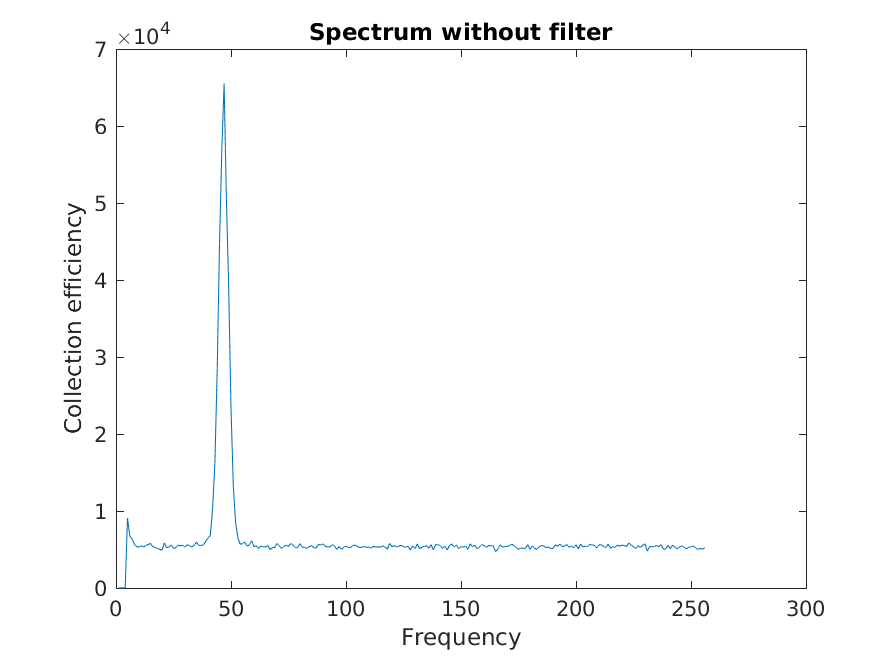
\includegraphics[width=1\linewidth]{../Exercises_and_Tasks/ex1/figures/spectra_nofilter.png}
  \caption{Raw spectrum}
  \label{fig:raw_spectrum}
\end{subfigure}
\begin{subfigure}{0.5\textwidth}
  \centering
  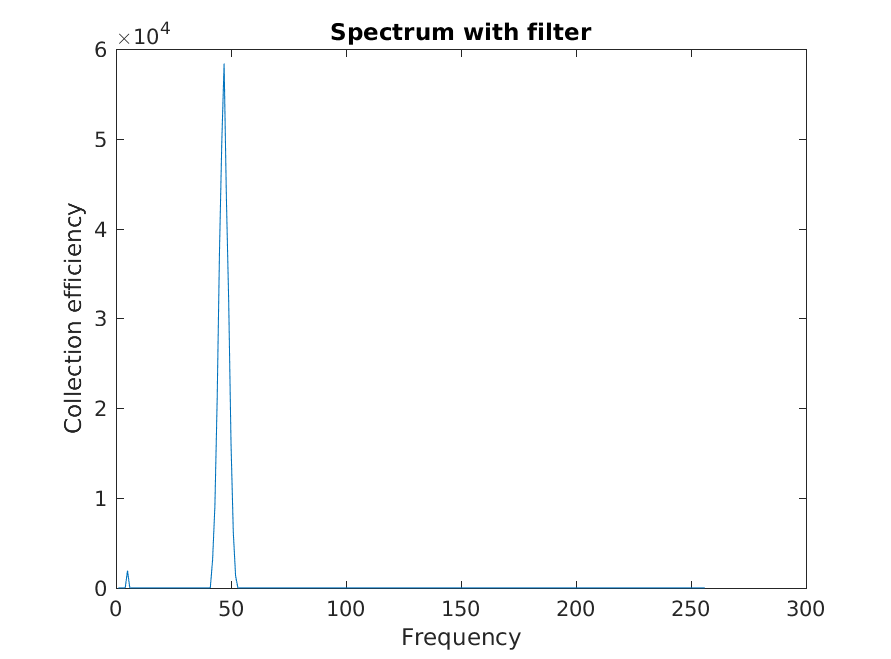
\includegraphics[width=1\linewidth]{../Exercises_and_Tasks/ex1/figures/spectra_noisecancelled.png}
  \caption{Spectrum cleaned from background noise}
    \label{fig:cleaned_spectrum}
\end{subfigure}
\end{figure}

\subsection{Calculate the Doppler frequency that each bin of the spectra corresponds to}
We received the spectra as histograms which are separated in 256 bins. The measured bandwith is $25\cdot10^6 $ Hz. Therefore each bin represents a frequency of
\begin{equation*}
 frequency = x * \frac{25\cdot10^6 Hz}{256}
\end{equation*}
where x is the bin number.
With the equations provided during the lecture we were also able to calculate the line-of-sight velocity.
The implementation in Matlab is shown in the following.\\

\begin{lstlisting}
for bin=1:256
    f_d(bin,1) = (bin-1)/bins*bandwith;
    v(bin,1) = f_d(bin,1) *lambda_0;
end;
\end{lstlisting}

\subsection{For each spectrum, define the peak location with the centroid
method}
The centroid method was introduced during the lecture and is defined as:
\begin{equation*}
f_{peak} = \frac{\int f_d \cdot p(f) df}{\int p(f) df}
\end{equation*}
Before we calculated the peak values we normalized our data to get a PDF instead of absolute values.
Since we are dealing with discrete values, we summed over all values in order to identify the peak value. 
In order to check all 312 $f_{peak}$ values, we first calculated the index of the maximum collection efficiency for each spectrum. The maximum should always represent the peak of the spectrum.
Next we determined the corresponding index of $f_{peak}$. Now we were able to compare the distance of the calculated indices. The results are shown in figure \ref{fig:failures}.

\begin{figure}[H]
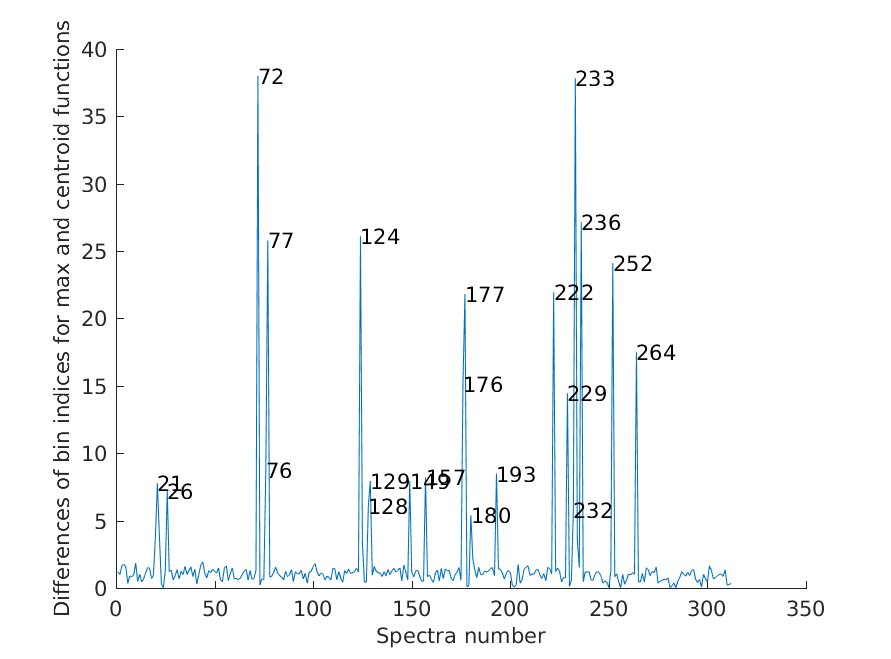
\includegraphics[width=1\linewidth]{../Exercises_and_Tasks/ex1/figures/failures.png}
\caption{Centroid Errors in bin distance}
\label{fig:failures}
\end{figure}

The figure shows that there are several errors. The centroid method fails for some spectra due to a measurement error. As stated in the exercise sheet the lidar was placed on the nacelle of a wind turbine. Therefore for some measurements the lidar might be blocked by the rotating blades which would result in a second frequency peak. If the spectrum contains two peaks, the centroid method returns the middle of these two peaks and is not applicable for this case.
One of those cases is shown in figure \ref{fig:measurement_error}.

\begin{figure}[H]
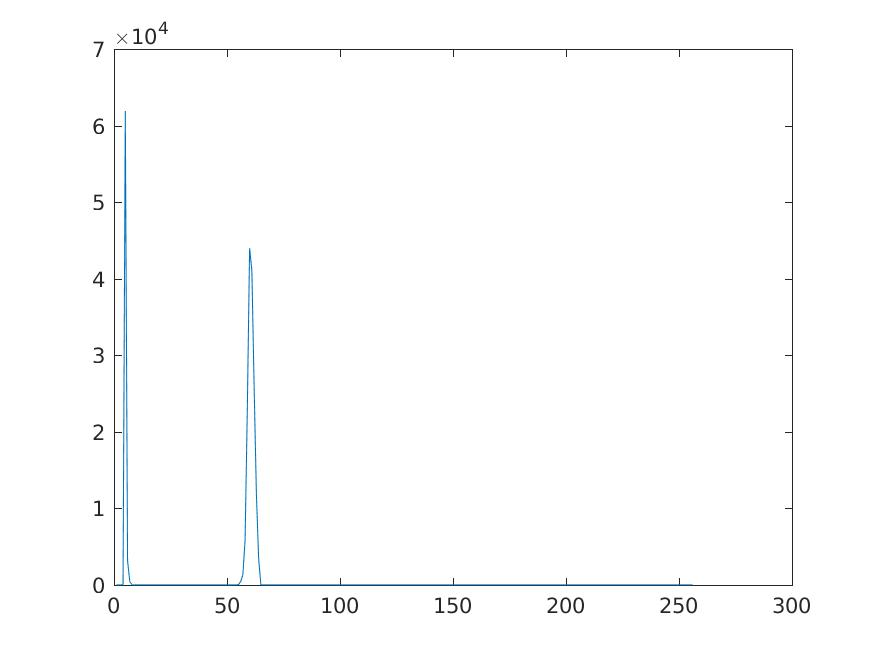
\includegraphics[width=1\linewidth]{../Exercises_and_Tasks/ex1/figures/spectra_noisecancels_normed_72.jpg}
\caption{Measurement error in spectrum 72}
\label{fig:measurement_error}
\end{figure}

\subsection{Correlate the calculated line-of-sight speeds}
In step 4 we were asked to correlate the calculated line-of-sight speeds with the lidar data itself. The correlation method was already provided. Therefore we only needed to calculate the line-of-sight velocity by multiplying $f_{peak}$ with $\lambda_0$. The resulting plot is shown in figure \ref{fig:correlation}. 

\begin{figure}[H]
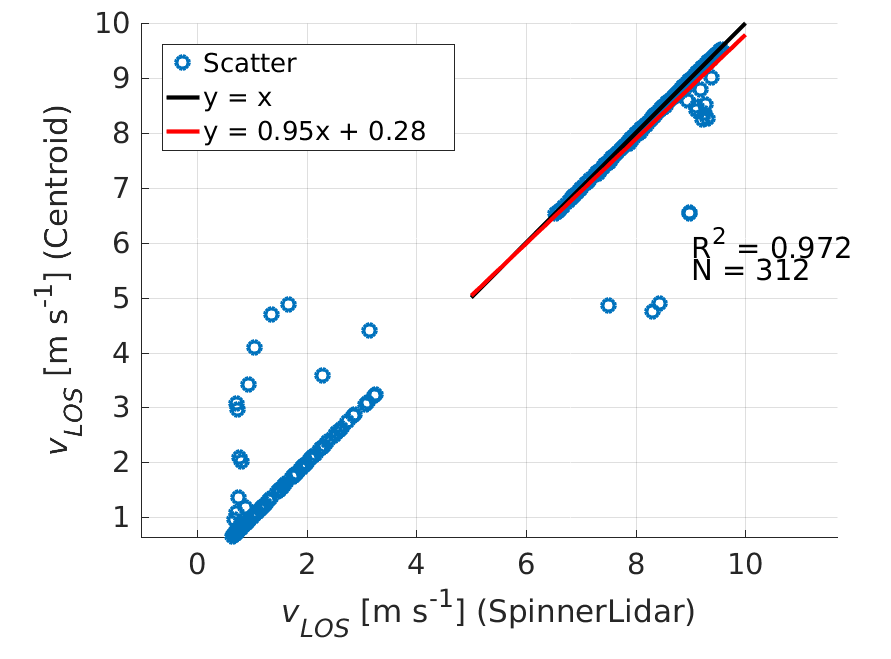
\includegraphics[width=1\linewidth]{../Exercises_and_Tasks/ex1/figures/correlation.png}
\caption{Correlation of the calculated line-of sight-speed and the lidar data}
\label{fig:correlation}
\end{figure}

Figure \ref{fig:correlation} shows a strong correlation of $R^2 = 0.972$. As discussed in section 1.3 there are measurement errors due to the position of the lidar. Some measurements are blocked by the moving blades. 
\section{VAD Scanning: from line-of-sight velocity to wind factor}
\subsection{Investigate the LiDAR data}
In exercise 2 we were working with a 6 hour dataset of VAD Lidar measurements located on the FINO1 platform. For further comparison we were also provided a 10 minute averaged dataset of FINO 1.
The first step was to filter bad measurements. A common procedure is to filter bad Carrier-to-Noise-Ratios (CNR). 
The procedure is shown in the following code-snippet:

\begin{lstlisting}
% Filter data by CnR, by setting to NaN and later in Step 2 discarding NaN
% values
cnr_ind = find(cnr_VAD <= -20 | cnr_VAD >= -5);
rs_VAD(cnr_ind) = NaN;
az_c_VAD(cnr_ind) = NaN;
\end{lstlisting}
After filtering the data we were asked to separate the data for the different range gates. We identified 14 different range gates, measuring at $61m, 64m, 67m, 70m, 72m, 75m, 78m, 81m, 84m, 87m, 90m, 93m, 96m$, and $98m$. 
The last task of 2.1 was to calculate the time for a full $360^\circ$ scan. The LiDAR has a scanner speed of $25^\circ/s$. Therefore one full scan takes:

\begin{align*}
\textit{time per scan} = \frac{360}{25^\circ/s} = 14.4s 
\end{align*}
The given data is measured at a time interval of 0.4 s. A full scan represents $14.4s / 0.4s = 36$ intervals.
\subsection{Separate the data single 360$^\circ$ scans and carry out a cosine fit}
The goal of this section is to compute the horizontal wind speed, the horizontal wind direction and the vertical wind speed. In the last section we calculated that a full scan is represented by 36 intervals. So in the ideal case of a homogeneous atmosphere the line-of-sight velocity should show a sine-like behaviour. There fore we should be able to fit this to a function of type:
\begin{equation*}
v_{rad} =  b \cdot\cos(\phi - \Theta) +a
\end{equation*}
where 
\begin{align*}
v_{hor} = \frac{b}{cos(\theta)} \hspace{1cm} w= \frac{-a}{\sin(\theta)} \hspace{1cm} D= b \pm 180
\end{align*}
To implement the fitting routine in Matlab we first defined the function, depending on the three parameters $b, \Theta$ and $a$ and the azimuth angle $\phi$. During the lecture the function $lsqcurvefit()$ was recommended as the fitting routine. It should be noted, that the function is not able to deal with $NaN$ values. Therefore $NaN$ values had to be discarded temporally.
The following code-snippet shows the Matlab implementation. The fitting was done over all full 360$^\circ$ scans and over all range gates.

\begin{lstlisting}
for j = 1:14 % number of Range Gates
    for i = 1:numberOfScans
        phi = az_c_VAD_filter((i-1)*intervalls_per_scan+18:(i-1)*intervalls_per_scan+53,j);
        v_r = rs_VAD_filter((i-1)*intervalls_per_scan+18:(i-1)*intervalls_per_scan+53,j);
        nanIndices = isnan(phi) | isnan(v_r); 
        phi(nanIndices) = [];
        v_r(nanIndices) = [];
        if length(phi>0)
            fitparam = lsqcurvefit(VADCos, startvalues, phi, v_r);
            savedparam{i,j} = fitparam;
            %calculate horiz and vertical speed
            v_hor = fitparam(1) / cosd(60);
            v_ver = -fitparam(3) / sind(60);
            D = abs(fitparam(1)-180);
            calc_times(i,j) = ts_VAD_filter((i-1)*intervalls_per_scan+18,j);
            calc_vHor(i,j) =  v_hor;
            calc_vVer(i,j) = v_ver;
            calc_D(i,j) = D;
        end
    end 
end
\end{lstlisting}

In order to understand what the fitting routine returns, we also plotted the data and the fitted curve. The results are shown in figure \ref{fig:fit}.

\begin{figure}[H]
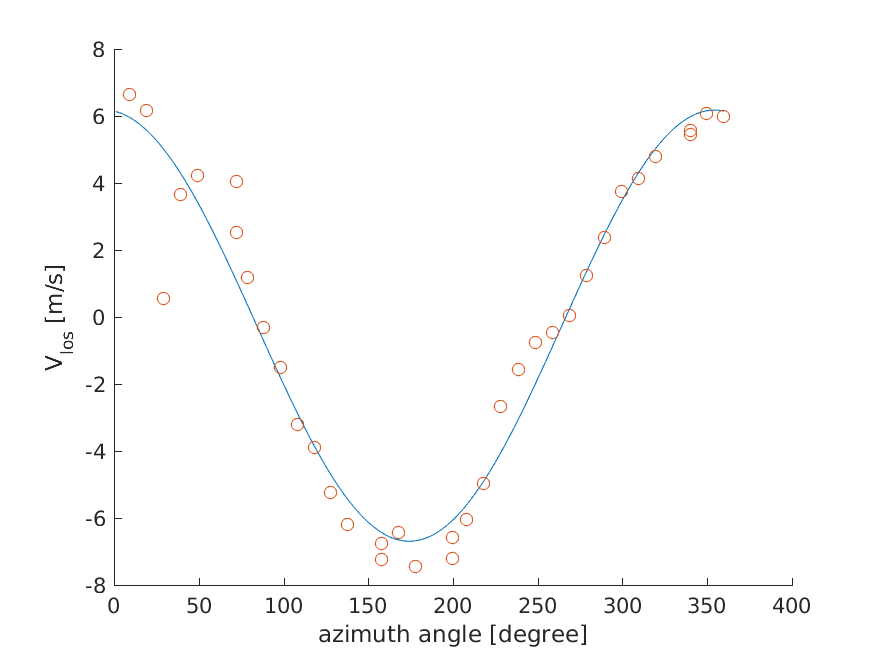
\includegraphics[width=1\linewidth]{../Exercises_and_Tasks/ex2/figures/fit.png}
\caption{Full 360$^\circ$ for Range Gate = 61 m with fit}
\label{fig:fit}
\end{figure}

\subsection{10 minute averages and comparison of vertical wind profiles and wind directions}
The FINO 1 data includes wind vanes at heights of \textit{33m, 40m, 50m, 60m, 70m, 80m, 90m} and eight anemometers at heights \textit{33m, 40m, 50m, 60m, 70m, 80m, 90m and 100m}.The measurements are in 10 minute intervals. The LiDAR data was measured at heights \textit{67m, 70m, 72m, 75m, 77m, 80m,	83m} and \textit{85m}.
To compare the vertical profiles we had to compute 10 minute averages of the LiDAR wind speeds and wind directions. Since we only had a six hour dataset we searched for the corresponding time stamp in the FINO 1 data. After averaging the LiDAR data and extracting the correct FINO 1. We were now able to compare the datasets. 
In Exercise 2 - Energy Meteorology we identified the logarithmic wind speed profile as a good method to predict the vertical wind speed profile.
Therefore we fitted the calculated LiDAR data and the given FINO 1 data with the help of logarithmic wind speed profile. 
The procedure for FINO 1 is shown following code-snippet:
\begin{lstlisting}
logProfileModel = @(b,z) b(1)/0.4 *(log(z/b(2)));
opts = statset('nlinfit');
opts.RobustWgtFun = 'bisquare';
logProfileCoeffsFino = real(nlinfit([33,40,50,60,70,80,90,100],...
avg_horSpeed_Fino,logProfileModel,[0.1,10^-5],opts));
\end{lstlisting}
The results are shown in figure \ref{fig:verticalprofiles} :
\begin{figure}[H]
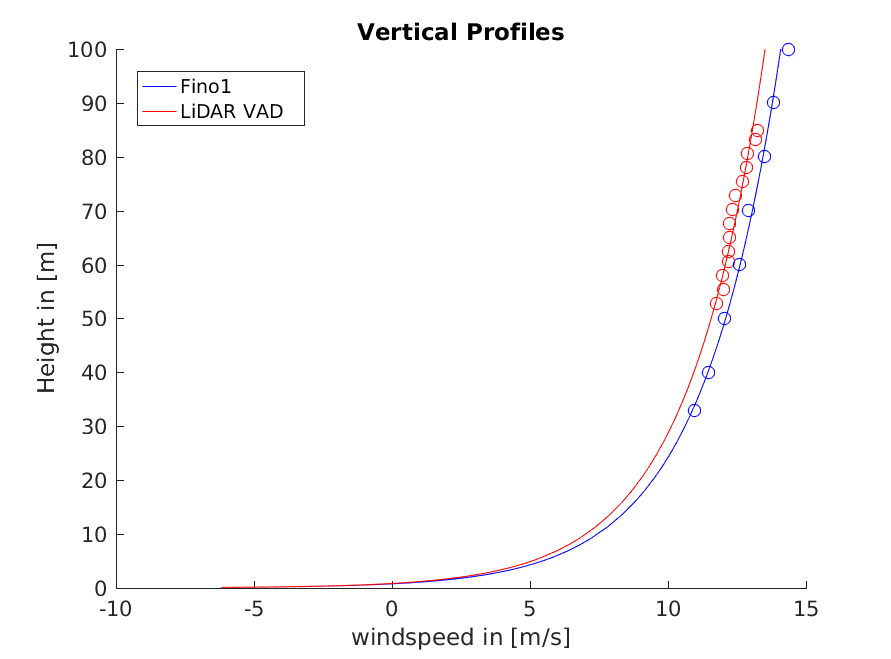
\includegraphics[width=1\linewidth]{../Exercises_and_Tasks/ex2/figures/verticalProfiles.png}
\caption{Vertical profile of FINO 1 and LiDAR measurement}
\label{fig:verticalprofiles}
\end{figure}
The figure shows that the vertical profile of the LiDAR is shifted to the left. As discussed in the lecture, anemometers measure more accurately and therefore the FINO 1 curve should be more representative. 

Further we evaluated the wind directions. For better comparison , we used measurements at similar heights. We used the already existing WindRose.m routine. The wind rose helps to evaluate and compare the wind directions.

In order to obtain correct wind directions we used the following plot routine:\\
\begin{lstlisting}
WindRose(fino_90_dir_interval,fino_speeds(:,7),'AngleNorth',0,'AngleEast',90,'freqlabelangle',45,'MaxFrequency',6);
WindRose(tenMinAvg_direction(:,7), tenMinAvg_horSpeed(:,7),'AngleNorth',0,'AngleEast',90,'freqlabelangle',45,'MaxFrequency',6);
\end{lstlisting}

The comparison between the two wind roses are shown in figure~\ref{fig:WindrosesVal}. 

\begin{figure}[htb!]
\label{fig:WindRose1_valdidation}
\begin{subfigure}{0.5\textwidth}
  \centering
  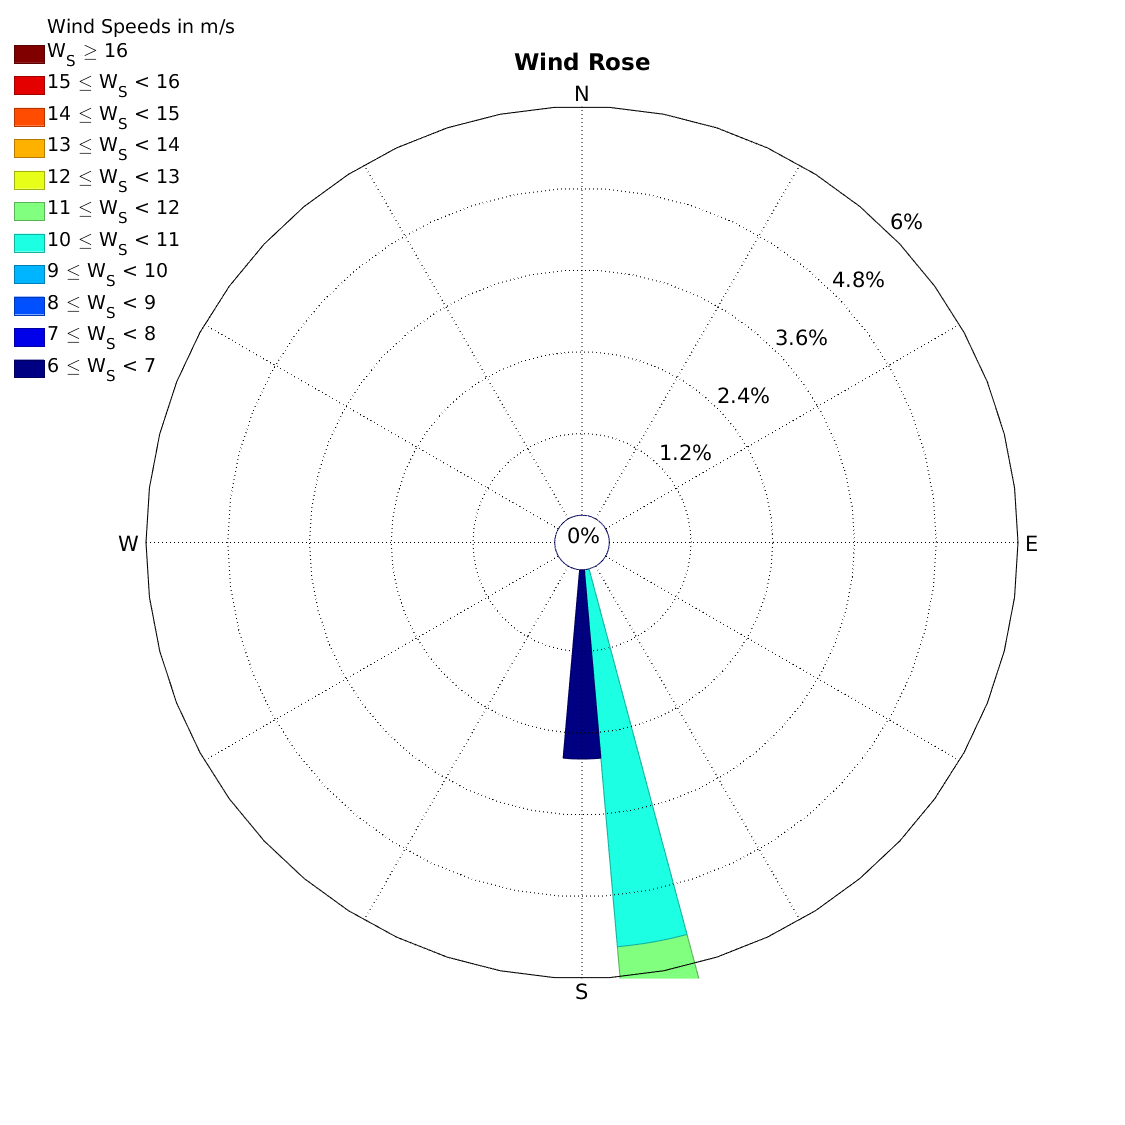
\includegraphics[width=1\linewidth]{../Exercises_and_Tasks/ex2/figures/WindRose_Fino1.png}
  \caption{Wind rose of FINO 1}
\end{subfigure}
\begin{subfigure}{0.5\textwidth}
  \centering
  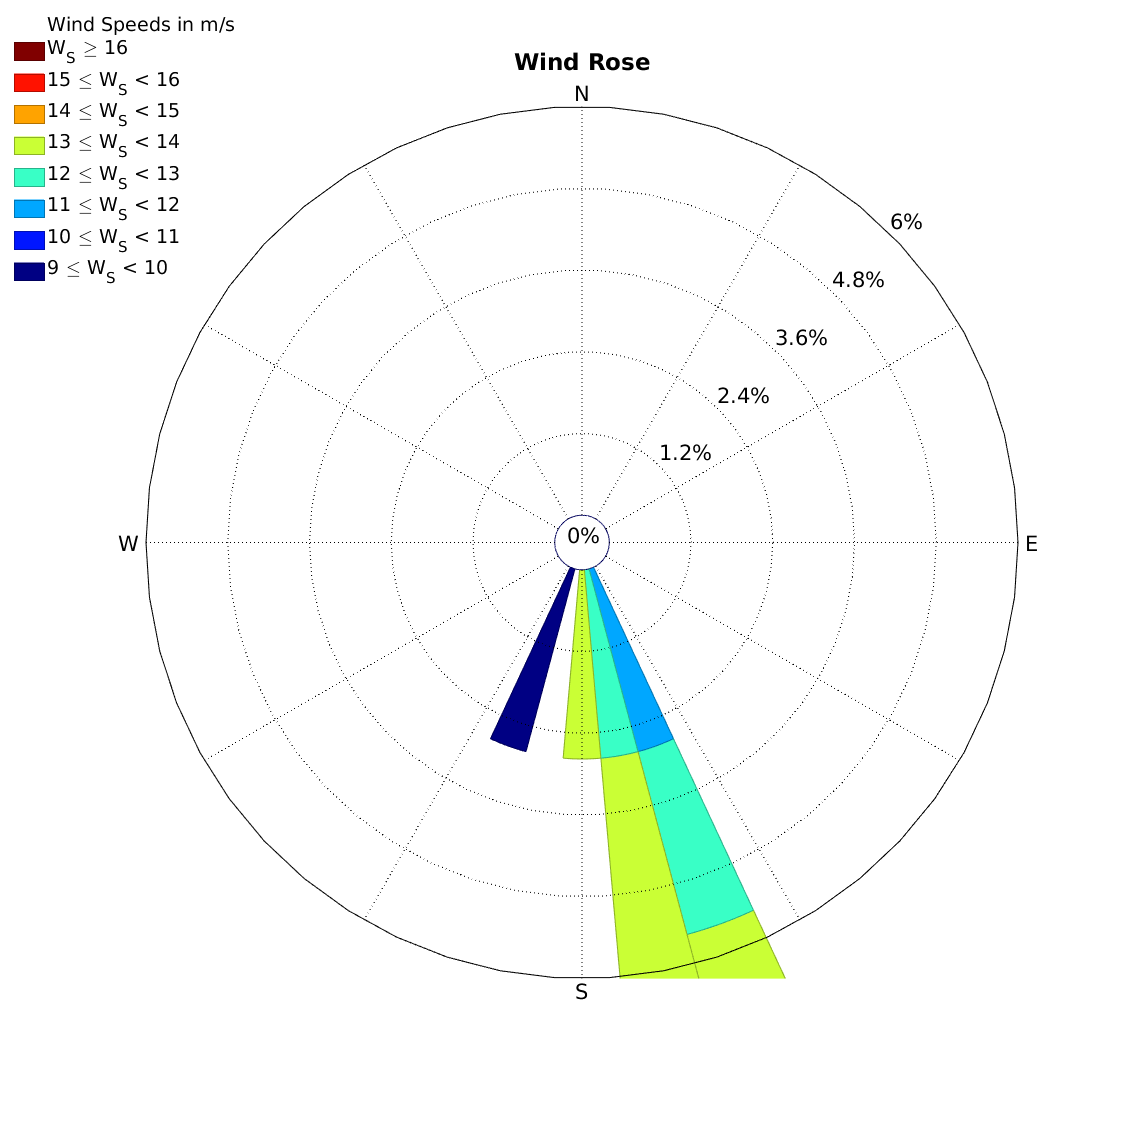
\includegraphics[width=1\linewidth]{../Exercises_and_Tasks/ex2/figures/WindRose_lidar.png}
  \caption{Wind rose of LiDAR VAD}
\end{subfigure}
\caption{Comparison of wind roses}
  \label{fig:WindrosesVal}
\end{figure}

We identify that there is noticeable shift in the wind directions from FINO 1 to the LiDAR VAD. If we only compare the 10-minute direction intervals the shift can be estimated to around 20$^\circ$. One reason for the shift might be that we assume a homogeneous wind field. In reality we deal with fluctuations that influence the measurements. 

\section{Multi-Lidar 3D vector reconstruction: from three line-of-sight velocities to 3D wind vector}
In this task we were provided a data set of about 90 minutes, measured by three short range WindScanners of the Technical University of Denmark. T
\subsection{Data structure}
he lidar data contains the 3D coordinates of each lidar system and the measured line-of-sight velocities. The three Lidars were focussed at the same measurement point at 90 meters height. The staring point was also give in 3D coordinates.
 The measurement setup is shown in figure~\ref{fig:measurementsetup}.

\begin{figure}[H]
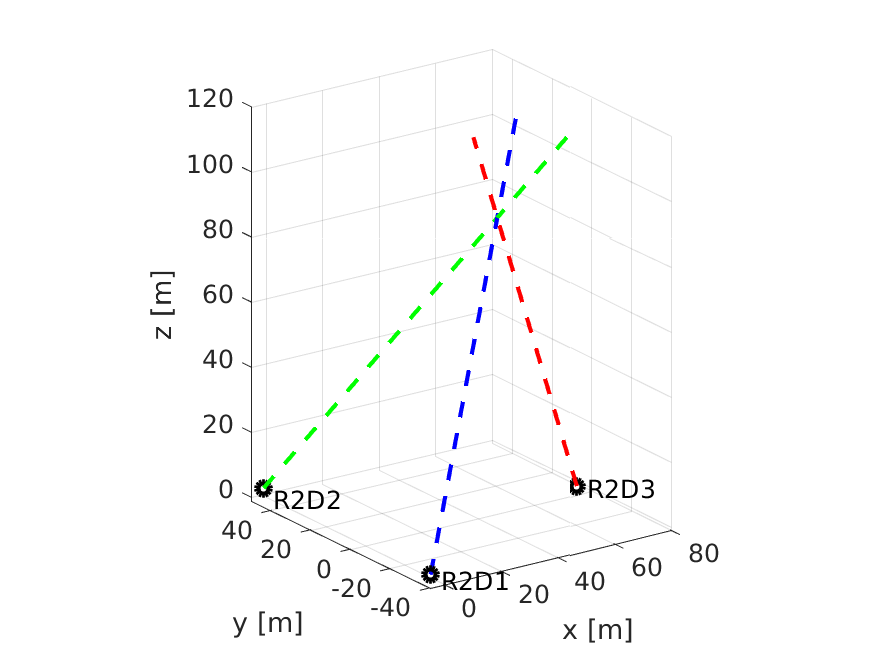
\includegraphics[width=1\linewidth]{../Exercises_and_Tasks/lidar.png}
\caption{Measurement setup}
\label{fig:measurementsetup}
\end{figure}
\subsection{Azimuth and elevation angle for each lidar}
In order to calculate the the azimuth and the elevation we used the geometric set-up of the system.
It should be noted that $0^\circ$ azimuth angle is defined to be aligned with the positive x-axis and is counted counter-clockwise for positive values. 
To Matlab implementation is shown below:\\

\begin{lstlisting}
for i=1:3
    distOnGround = sqrt((staring_point(1) - lidar_positions(1,i))^2+(staring_point(2) - lidar_positions(2,i))^2);
    distDiagonal = sqrt(distOnGround^2 + (staring_point(3) - lidar_positions(3,i))^2);
    ele(i) = acosd(distOnGround/distDiagonal);
    azi(i) = atand((staring_point(2)-lidar_positions(2,i))/(staring_point(1)-lidar_positions(1,i)));
end

azi(3) = azi(3) + 180
\end{lstlisting}

The resulting angles are shown in the following table:\\

\begin{tabular}{c||c|c|}
& elevation angle in $^\circ$& azimuth angle in $^\circ$\\
\hline
Lidar 1 &56.6 & 35.93 \\
Lidar 2 &51.92 & -46.04\\
Lidar 3 & 70.38& 189.61\\
\end{tabular}
\subsection{Matrix system that converts the three line-of-sight velocities to the u,v and w components}
To calculate the three components of the line-of-sight velocities we had to set up a linear equation system in the form of $[A] \cdot b = c$. 
Each measured line of sight velocity is defined as:
\begin{equation*}
V_{rad} = [u, v ,w]\cdot[\cos(\beta)\sin(\alpha), \cos(\beta)\cos(\alpha), \sin(\beta)]
\end{equation*}
That leaves us with 3 equation for 3 unknown. 
The trigonometric functions represent the coefficient matrix A and the three different line of sight velocities $V_{rad}$ represent c.
To solve for $[u,v,w]$ we have to multiply $A^{-1}$ with the radial wind speed vector.
In Matlab this can be done with $mldivide()$:

\begin{lstlisting}
    solution = mldivide(matrix, V(i,:)');
    %solution = inv(matrix)*V(i,:)';
    u(i,1) = solution(1);
    v(i,1) = solution(2);
    w(i,1) = solution(3);
end
\end{lstlisting}

The calculated $\theta$ and $\delta$ are $0,089$ and $-0,022$.
\subsection{Statistics}
In the last section, the lidars are aligned with the main wind direction  such that both v and w have a mean of 0 m/s. After that the mean and the standard deviation for each of the 3 lidars are calculated. The results are shown in the following table.\\

\begin{tabular}{c||c|c|}
& $\mu$& $\sigma$\\
\hline
Lidar 1 &-4.83 & 0.76 \\
Lidar 2 &-3.20 & 0.63\\
Lidar 3 & 	3.38& 0.96\\
\end{tabular}
\end{document}